\documentclass[a4paper, 10pt]{report}
\usepackage[italian]{babel}
\usepackage[T1]{fontenc}
\usepackage[utf8]{inputenc}
\usepackage{charter}
\usepackage{amsmath}
\usepackage{amsthm}
\usepackage{amsfonts}
\usepackage{graphicx}
\usepackage{wrapfig}
\usepackage{tcolorbox}
\usepackage{fancyhdr}
\usepackage{listings}

\usepackage{geometry}
\geometry{a4paper, left=2cm,right=2cm,top=2cm,bottom=2cm}

\pagestyle{fancy}
\lhead{}
\chead{}
\rhead{\bfseries 29 ottobre 2019 }
\lhead{\bfseries Linguaggi}

\begin{document}

\paragraph*{Tempi di bindings} I bindings possono essere creati:
\begin{itemize}
\item[-] A tempo di compilazione (early binding), ottenendo un'esecuzione più veloce ma un programma poco flessibile in quanto l'allocazione della memoria è statica (uso dello stack). Quindi tutti  i bindings hanno indirizzi assoluti;
\item[-] A tempo di esecuzione (late binding), ottenendo un'esecuzione più lenta ma un programma più flessibile grazie all'allocazione dinamica della memoria. Tutti i bindings, quindi, hanno indirizzi non assoluti.
\end{itemize}
Esistono linguaggi che adottano entrambe le soluzioni.\\

\noindent ATTENZIONE: affinchè un identificatore abbia significato, deve essere legato a qualcosa.

\subsection*{Semantica delle dichiarazioni}
Per riferire gli oggetti denotabili (valori riferibili tramite identificatore) usiamo il concetto di \textbf{ambiente}, che indica l'insieme delle associazioni tra nomi e oggetti denotabili esistenti a runtime in uno specifico punto del programma ed in uno specifico momento dell'esecuzione.

Le associazioni vengono create nell'ambiente tramite le \textbf{dichiarazini}. Infatti queste permettono di passare da free-occurrences, ovvero occorrenze di uso senza legame, ad applied-occurrences, dove l'identificatore non è più libero.

\paragraph*{Identificatori liberi} Un identificatore è libero se non c'è nessuna dichiarazione che lo coinvolge. 
\begin{tcolorbox}[title=\textbf{Definizione per induzione}]
La funzione $FI : Exp \rightarrow Id$ che associa ad ogni espressione l'insieme degli identificatori liberi in essa contenuti è definita come segue:\\
$
FI(k) = \emptyset\\
FI(id) = \{id\}\\
FI(e_0 \hspace{0.1cm} bop \hspace{0.1cm} e_1) = FI(e_0)\cup FI(e_1)\\
FI(not \hspace{0.1cm} e) = FI(e)
$
\end{tcolorbox}

\paragraph*{Termine chiuso} In un linguaggio, un termine (programma) in cui non ci sono identificatori liberi è detto chiuso.

\paragraph*{Termine groud} In un linguaggio, un termine (programma) in cui non ci sono identificatori è detto ground.

\paragraph*{Ambiente dinamico} Un ambiente dinamico è un elemento dello spazio di funzioni
\begin{align*}
Env = \cup_{V \subseteq_f Id} Env_V
\end{align*}
dove $Env_V : V \rightarrow DVal$ e $\cup\{\perp\}$ ha metavariabile $p$.

\begin{center}
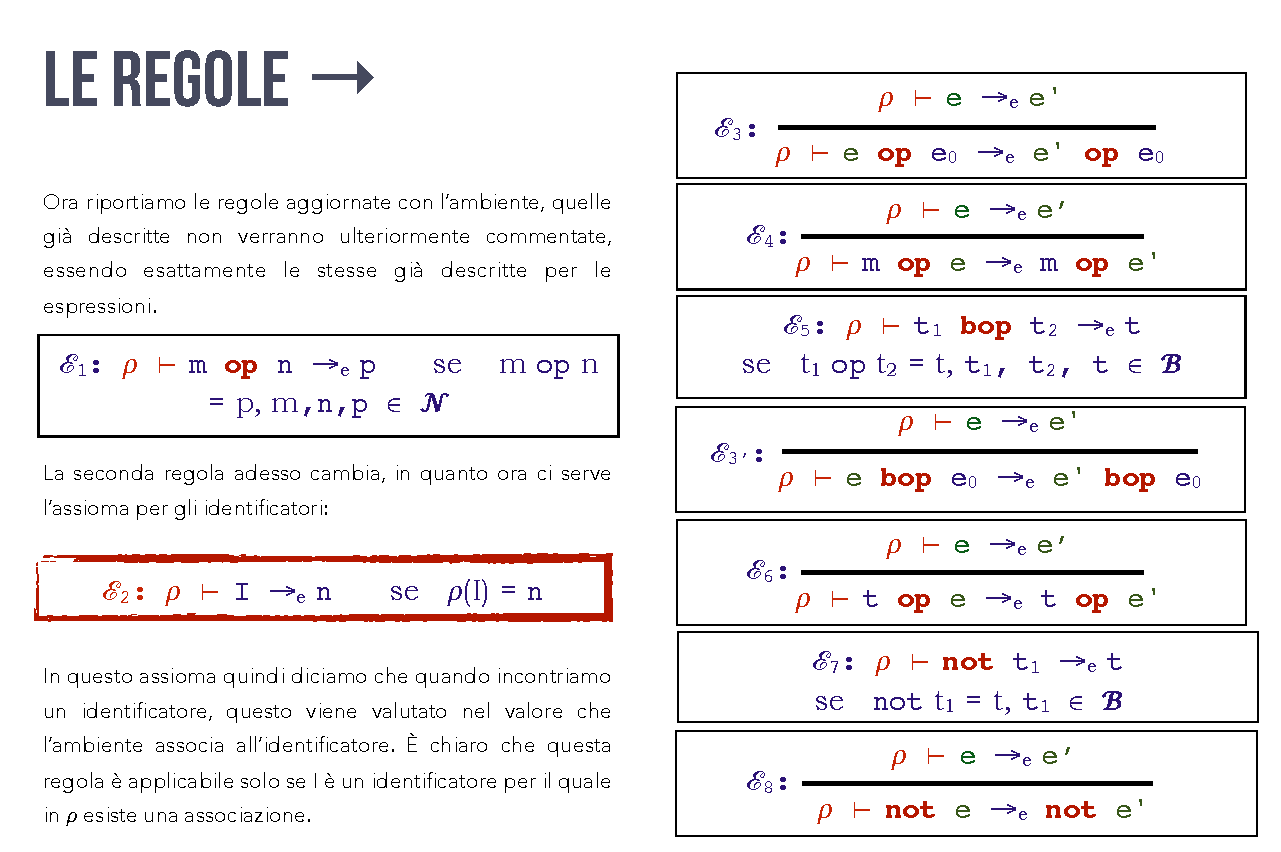
\includegraphics[scale=0.8]{regole.pdf}
\end{center}


\end{document}